\documentclass[prl,aps,10pt,twocolumn,showkeys,nofootinbib]{revtex4-1}
\def\baselinestretch{0.98}

%\usepackage[normalem]{ulem}
%\usepackage{jheppub}
\usepackage{amsmath,amssymb,amsfonts,amsthm}
\usepackage{amsbsy} 
\usepackage{epsfig}
\usepackage{latexsym}
\usepackage{color}
\usepackage[utf8]{inputenc}
\input amssym.def
\input amssym.tex
%\usepackage{showlabels}

\usepackage{hyperref}

\newcommand{\oarX}[1]{\href{http://arxiv.org/abs/#1}{{\ttfamily #1}}}
\newcommand{\arX}[1]{\href{http://arxiv.org/abs/#1}{{\ttfamily arXiv:#1}}}
\newcommand{\doin}[2]{\href{http://dx.doi.org/#1}{#2}}
\newcommand{\Eq}[1]{(\ref{#1})}

%%%%%%%%%%%%%%%% Definitions %%%%%%%%%%%%%%%%%%%
\def\barr{\begin{array}}
\def\earr{\end{array}}
\def\half{\frac{1}{2}}
\def\ben{\begin{equation}}
\def\een{\end{equation}}
\def\bs{\begin{subequations}}
\def\es{\end{subequations}}
\def\bena{\begin{eqnarray}}
\def\eena{\end{eqnarray}}
\def\mathgrave{\mathaccent"7012} 
\def\mathacute{\mathaccent"7013} 
\def\vol{\rm Vol}
\def\const{{\rm constant}}
\def\bR{\mathbb{R}}
\def\bC{\mathbb{C}}
\def\bZ{\mathbb{Z}}
\def\SO{{\rm SO}}
\def\O{{\rm O}}
\def\GL{{\rm GL}}
\def\SU{{\rm SU}}
\def\SL{{\rm SL}}
\def\GG{\mathfrak{G}}
\def\Sp{{\rm Spin}}
\def\cV{{\cal V}}
\def\im{{\rm i}}
\def\cc{{\rm c.c.}}
\def\cK{{\cal K}}
\def\M{\mathcal{M}}
\def\be{\begin{equation}}
\def\ee{\end{equation}}
\newcommand{\ie}{\textit{i.e.}~}
\newcommand{\eg}{\textit{e.g.}~}
\def\bes{\begin{eqnarray}}
\def\ees{\end{eqnarray}}

\newcommand{\hchi}{\hat{\chi}}
\newcommand{\ha}{\hat{a}}
\newcommand{\had}{\hat{a}^{\dagger}}

\newcommand{\dd}{\mathrm{d}}

\newcommand{\qq}[1]{\emph{#1}}

\newcommand{\lie}{\mathfrak{g}}
\newcommand{\Tr}{\mathrm{Tr}}

\newcommand{\bra}[1]{\left\langle #1 \right|}
\newcommand{\ket}[1]{\left| #1 \right\rangle}
\newcommand{\hphi}{\hat{\varphi}}
\newcommand{\hphid}{\hat{\varphi}^{\dagger}}
\newcommand{\perm}{\text{permut.}}
\def\DD{{\mathrm{D}}}

%%%%%%%%%%%%%%%%%%%%%%%%%%%%%%%%%%%%%%%%%%%%%%%%
\begin{document}


\title{Shocks in the Early Universe}


\author{Ue-Li Pen }
\affiliation{Canadian Institute for Theoretical Astrophysics, 60 St George St, Toronto, ON M5S 3H8, Canada}

\author{Neil Turok}
\affiliation{Perimeter Institute for Theoretical Physics, Waterloo ON N2L 2Y5, Canada}


\date{\today}

%%%%%%%%%%%%%%%%%%%%%%%%%%%%%%%%%%%%%%%%%%%%%%%%%%%%%%%

\begin{abstract}
We point out a surprising consequence of the usually assumed initial conditions for cosmological perturbations. 
Namely, a scale-invariant spectrum of Gaussian, linear, adiabatic, scalar, growing mode perturbations not only creates acoustic oscillations, of the kind observed in great detail on large scales today, it also leads to the production of shock waves in the radiation fluid of the very early universe. At very early epochs, $1$ GeV$<T<10^{7}$ GeV, assuming standard model physics, viscous damping is negligible and nonlinear effects turn acoustic waves into shocks after $\sim 10^4$ oscillations. The resulting scale-invariant network of shocks provides a natural mechanism for creating significant departures from local thermal equilibrium as well as primordial vorticity and gravitational waves. 
\end{abstract}

% \pacs{98.80.-k,~98.65.-r,~98.80.Cq,~95.36.+x}

\maketitle

Over the past two decades, observations have lent powerful support to a strikingly simple model of the early universe: a flat, radiation-dominated Friedmann-Lema\^{i}tre-Robinson-Walker (FLRW) background cosmology, with a nearly scale-invariant spectrum of small-amplitude, Gaussian-distributed, growing mode primordial perturbations. These perturbations caused the cosmic background anisotropies, mapped in fine detail by the WMAP and Planck satellites. They also seeded the distribution of galaxies, traced in large scale structure surveys. In this Letter we explore their evolution on very small scales and at very early times.  

At first sight, the evolution of linear perturbations deep in the radiation-dominated epoch might seem trivial. As they enter the Hubble radius perturbations start to oscillate, with an amplitude $\epsilon \sim10^{-4}$. It might seem reasonable to describe such modes within linear theory, according to which they simply redshift away as the universe expands. However, higher order perturbative calculations \cite{Gielen} revealed that the situation is actually far more interesting. As we shall explain, non-linear effects cause the waves to steepen and form shocks, after they have undergone $\epsilon^{-1} \sim 10^{4}$ oscillations. We have studied this phenomenon in detail through detailed numerical simulations in one, two and three dimensions: movies and other supplementary materials are provided on the website \cite{weblink}. 

In a perfect fluid, entropy is conserved. The presence of acoustic modes means that the entropy is lower than that of the homogeneous state but, within the perfect fluid description, there is no way for entropy to increase. However, due to nonlinear effects, the waves steepen to form shocks. Although the fluid equations fail at this point, the evolution of the system is still uniquely defined by the relevant local conservation laws. Within this description, shocks generate entropy and it is this process through which the maximum entropy, homogeneous, thermal equilibrium state is achieved. Not only do primordial shocks produce entropy, they also create vorticity, a process which is likewise forbidden by the perfect fluid equations. Both effects involve strong departures from local thermal equilibrium and are of potentially of relevance to many important early-universe questions including the generation of primordial magnetic fields and gravitational waves, and baryogenesis. These and other consequences of shocks in the early universe will be explored elsewhere~\cite{penturoklong}. 

Of course, the perfect fluid description is not an exact one, and dissipative processes are important on small scales.  In fact, the shock width $L_s$ is set by the shear viscosity $\eta$, and the density jump $\epsilon \rho$ across the shock. For a relativistic equation of state, {\it i.e.}, $P=c_s^2 \rho$, with the speed of sound $c_s=1/\sqrt{3}$, we find $L_s=9\sqrt{2}\,\eta/(\epsilon \rho)$ ~\cite{LL,penturoklong}. For shocks to form at all, $L_s$ must be smaller than the scale undergoing nonlinear steepening and shock formation, which is of order $\epsilon$ times the Hubble radius, $R_H=\sqrt{3} M_{Pl}\rho^{-\half}$, with $M_{Pl}\equiv(8 \pi G)^{-\half}$ the reduced Planck mass. Detailed calculations in the standard model \cite{moore} indicate that above the electroweak temperature, the right handed leptons, coupling mainly through weak hypercharge, dominate the viscosity, yielding $\eta\sim 16 /g'^4\ln(1/g') \sim 400 T^3$ for standard model content. Using $\rho=(\pi^2/30){\cal N} T^4$, with $N=106.75$ the effective number of degrees of freedom, we find $L_s$ falls below $\epsilon R_H$ and hence shocks can form, when $T$ falls below $\sim 10^{7}$ GeV.  Hence, for 
 temperatures $10^2$ GeV$< T <10^{7}$GeV the effects of viscosity may be neglected in the shock formation process. For example, at the electroweak temperature the shock width is $10^{-5}$ of the scale on which shocks form, so that viscous effects are utterly negligible both in shock formation and, as we shall discuss below, shock decay.  However, once $T$ falls below the electroweak scale and the Higgs field gains a vev $v$,  the neutrino mean free path grows very rapidly, as 
$\sim v^4/T^5$, exceeding the shock formation scale \cite{penturoklong} when $T$ falls below $\sim 1$ GeV. At lower temperatures, the primordial acoustic waves are damped away by neutrinos before they can steepen into shocks.

\begin{figure}[htp]
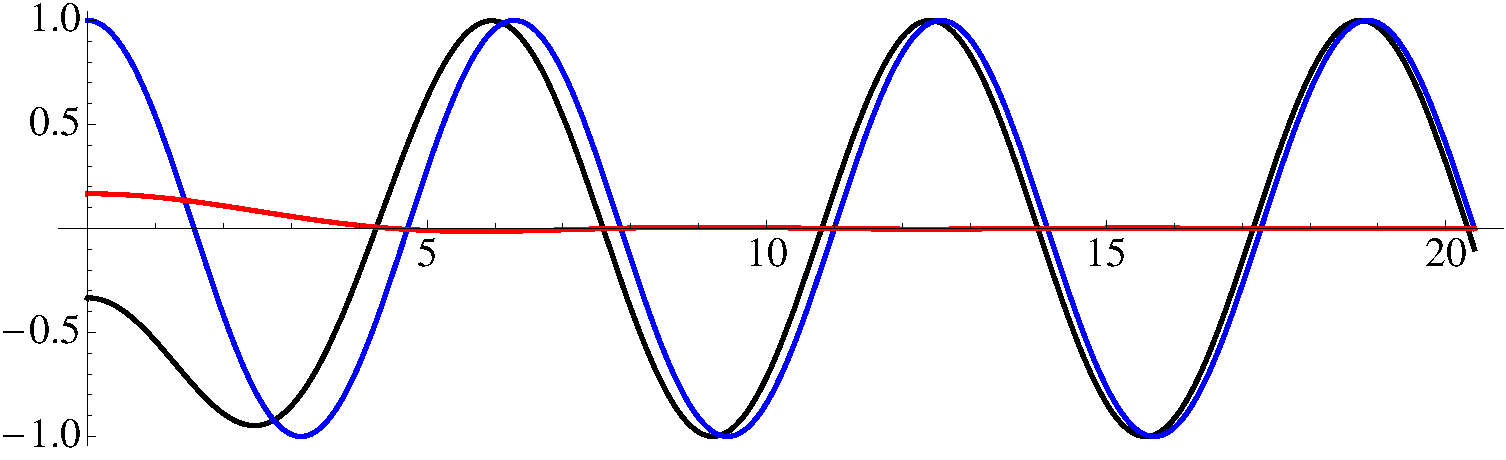
\includegraphics[scale=0.35]{modesfig.pdf}
\caption{The evolution of the growing mode linear perturbation, in a radiation-dominated universe, in conformal Newtonian gauge. The horizontal axis is $kt/\sqrt{3}$ where $k$ is the comoving wavenumber of the mode and $t$ is the conformal time. The black line shows the fractional density perturbation $\delta_k(t)$, and the red line the corresponding Newtonian potential $\Phi_k(t)$. The blue line shows the corresponding mode $\delta_k(t)$ in flat spacetime, which closely approximates the cosmological mode on sub-Hubble scales.}
\label{modesfig}
\end{figure}

This Letter is devoted to this early, radiation-dominated epoch in which shocks can form. We assume the standard, ``minimal", nearly scale-invariant perturbations. For each comoving wavenumber $k$ there are two scalar perturbation modes. One, the ``growing mode,'' is regular at the big bang singularity while the other, the ``decaying mode,'' diverges there. Vortical modes likewise diverge at the singularity. It is conventional (and very reasonable) to assume that the growing mode dominates as the universe emerges from its early moments. The evolution of this mode is illustrated in Fig. \ref{modesfig}: as its wavelength crosses the Hubble radius, the fluid starts to oscillate as a standing wave, and the associated metric perturbations decay. Once they become negligible, the fluid evolves as if it is in an unperturbed FLRW background. The tracelessness of the stress-energy tensor for perfect radiation means that the evolution of the fluid is identical, up to a trivial Weyl rescaling, to that in flat spacetime, where the conformal time $t$ and comoving coordinate $\vec{x}$ in the FRW line element are mapped to the usual Minkowski coordinates. 

In flat spacetime and for a constant equation of state, $P=c_s^2 \rho$, the fluid equations read $\partial_\mu T^{\mu \nu}=0$, where $T^{\mu \nu}=(1+c_s^2) \rho u^\mu u^\nu +c_s^2 \rho \eta^{\mu \nu}$, with $u^\mu=\gamma_{v}(1,\vec{v})$ the 4-velocity. In linear theory, the fractional density perturbation $\delta$ and velocity potential $\phi$ obey the continuity equation $\dot{\delta}=-(1+c_s^2) \vec{\nabla}^2 \phi$ and the acceleration equation $\dot{\phi}=-c_s^2/(1+c_s^2) \delta$. For cosmological growing mode initial conditions, we obtain for the sub-Hubble modes $\delta(t,\vec{x})=\sum_{\vec{k}} \delta^{(1)}_{\vec{k}} (t) e^{i\vec{k}.\vec{x}}$,  and similarly for $\phi(t,\vec{x})$ with $ ( \delta^{(1)}_{\vec{k}} (t) ,  \phi^{(1)}_{\vec{k}} (t) )\propto \bigl(\cos (k c_s t),-\sin (k c_s t)/(4 k c_s)\bigr).$ Thus, in linear theory, the perturbations are well-described by the correlator
\ben
\langle\delta^{(1)}_{\vec{k}}(t)\delta^{(1)}_{\vec{k}'}(t') \rangle=\delta_{\vec{k}+\vec{k}',\vec{0}}\,{2 \pi^2{ \cal A}\over k^3 V} \cos(k c_s t) \cos(k c_s t'),
\label{eq1}
\een
where ${\cal A}\equiv \epsilon^2$ is the variance per log interval in $k$ and $V$ is a notional comoving ``box'' larger than any scale of interest. The modes oscillate with angular frequency $\omega=c_s k$ where $c_s$ is the speed of sound. From Planck measurements, we determine $\epsilon\approx 6\times 10^{-5}$~\cite{foottilt}.

{\it Wave steepening:} 
The nonlinear fluid equations are $\partial_\mu T^{\mu \nu}=0$, where $T^{\mu \nu}=(1+c_s^2) \rho u^\mu u^\nu +c_s^2 \rho \eta^{\mu \nu}$, with $\rho$ the fluid energy density and $u^\mu=\gamma_{v}(1,\vec{v})$ the 4-velocity.  $T^{\mu \nu}$ depends on four independent variables, $\rho$ and $\vec{v}$. Hence, the spatial stresses $T^{ij}$ may be expressed in terms of the four $T^{\mu 0}$: expanding in $T^{0i}/\overline{T^{00}}$, we obtain $T^{ij}\approx c_s^2 T^{00}\delta^{ij} +(T^{i 0}T^{j 0}-c_s^2\delta^{ij} T^{0k} T^{0k})/((1+c_s^2)\overline{T^{00}})+\dots$. In this way, the four equations, $\partial_\mu T^{\mu \nu}=0$ completely determine the evolution of the fluid. 

A standing wave may be viewed as a sum of a left-moving and a right-moving wave, of half the amplitude. The formation of shocks is easiest to see if we follow one of these waves. Assuming planar symmetry, and that the wave is  moving in the positive $x-$direction, we define the dimensionless momentum density $\Pi\equiv T^{01}/\overline{T^{00}}$, where the overline denotes spatial average. Then to second order in $\Pi$, the fluid equations imply $8 c_s \partial_u \partial_v \Pi +(\partial_u^2-\partial_v^2)\Pi^2=0$, where $u\equiv x-c_s t$ and $v=x+c_s t$. At linear order, we have a right-moving wave $\Pi^{(1)}(u)$. The equation of motion implies that $v$ derivatives are suppressed relative to $u$ derivatives by one power of the perturbation amplitude. Hence we can drop the $\partial_v^2\Pi^2$ term and integrate once in $u$ to obtain as the effective equation for $\Pi(v,u)$, valid up to second order,
\be
4 c_s
\partial_v \Pi + \Pi \partial_u \Pi=0.
\label{eq2}
\ee
This is Burger's equation, a well-known model exhibiting shock formation: generic smooth initial data $\Pi(0,u)$ develops discontinuities in finite time $v$. 

The wave steepening effect is readily seen in perturbation theory. Consider, for example, a right-moving mode with $\delta^{(1)}=-{1\over 2} \epsilon \sin (k u)$. From local energy conservation, it follows that $\Pi^{(1)}=-{1\over 2}  c_s \epsilon \sin (k u).$  From (\ref{eq2}) one then finds at second order $\Pi^{(2)}=-c_s \epsilon^2 (k v/32) \sin (2 k u)$. Rewriting the solution in terms of $x$ and $t$, one sees the second order term causes a ``steepening'' of the solution around, for example, the zero at $u=0$, {\it i.e.}, $x=c_s t$, with the second order contribution to the gradient $\partial_x \Pi$ equalling the first order contribution at $t=4/(k c_s \epsilon)$, signalling the breakdown of linear perturbation theory at that time. In fact, equation (\ref{eq2}) may be solved exactly by the method of characteristics. In this method, one shows that the solution propagates along straight lines, so that $\Pi(v,u+\Pi(0,u) v/(4 c_s))=\Pi(0,u)$, where $\Pi(0,u)$ is initial data at $v=0$. The characteristic lines first intersect at $u=0$ and $v=4 c_s/k$, demonstrating that shocks indeed form precisely at $t=4/(k c_s \epsilon)$, {\it i.e.}, after $2/(\pi \epsilon)$ oscillation periods of the original linear wave. 

{\it Characteristic rays:} In more general, higher-dimensional situations, we may gain insight into shock formation by computing characteristic rays, {\it i.e.}, the trajectories followed by short-wavelength, small amplitude disturbances~\cite{LL}. Such rays may be used to define characteristic surfaces whose degeneration signals the formation of shocks. In a relativistic fluid the 3-vorticity may be defined as $\vec{\nabla}\wedge (h \vec{u})$, where $h$ is the enthalpy density (for $P={1\over 3} \rho$, $h\propto \rho^{1\over 4}$). If the vorticity is initially zero, as for cosmological perturbations, then it remains zero as long as the fluid equations are valid. Hence we may write $h \vec{u}=\vec{\nabla} \phi$, with $\phi$ a potential, at least until shocks form. We write the perturbed density and potential as follows: $\rho=\overline{\rho}(1+\delta_b+d \delta)$ and  $\phi=\delta \phi_{b}+ d\phi$, where $\delta_{b}$ and $\delta \phi_{b}$ represent a background of linearized waves and $d \delta$ and $d \phi$ represent the additional short-wavelength characteristic ``tracers.'' Assuming $c_s=1/\sqrt{3}$, the  evolution of $d \delta $ and $d \phi$ is governed by the equations $\partial_t d \delta+{4\over 3} \vec{\nabla}^2 d \phi +{1\over 3} \vec{\nabla}\cdot (\delta_{b}\vec{\nabla}d\phi+d \delta \,\vec{\nabla}\phi_{b} )=0$ and $\partial_t d \phi +{1\over 4} d \delta  - {1\over 16} \delta _{b} d\delta+\vec{\nabla}\phi_{b}\cdot\vec{\nabla} d\phi=0$. These equations are solved in the stationary phase approximation: we set $d\phi=A_\phi e^{i {S}}$ and $d\delta=A_\delta e^{i {S}}$ and assume that $A_\phi$ and $A_\delta$ vary slowly so that the variation of the phase $S$ controls the wave fronts. The leading (imaginary) part of the equations of motion yields a linear eigenvalue problem for $A_\phi$ and $A_\delta$, with $i\partial_t S$ the eigenvalue.  We obtain
\ben
\partial_t  { S}=-{\sqrt{\vec{(\nabla}S)^2}\over \sqrt{3}}-{2\over 3} (\vec{\nabla}S \cdot\vec{\nabla}\phi_{b}),
\label{eq4}
\een
the Hamilton-Jacobi equation for a dynamical system with Hamiltonian ${\cal H}(\vec{p},\vec{x},t) =-\partial_t  {S}(t,\vec{x})$, where ${ S}(t,\vec{x}(t))$ is the action calculated on a natural path, {\it i.e}, a solution of the equations of motion. The Hamiltonian
\ben
{\cal H}(\vec{p},\vec{x},t) ={|\vec{p}\,|\over \sqrt{3}}+{2\over 3} \vec{p} \cdot\vec{\nabla}\phi_{b}(t,\vec{x})
\label{eq5}
\een
and the ray trajectories $\vec{x}(t)$ obey Hamilton's equations:
\ben
\dot{\vec{x}}={\vec{n}\over \sqrt{3}} +{2\over 3} \vec{\nabla}\phi_{b}, \quad \dot{n_i}=-{2\over 3} (\partial_i-n_i(n_j\partial_j))(\vec{n}\cdot \vec{\nabla}\phi_{b}),
\label{eq6}
\een
where $\vec{n}\equiv \vec{p}/|\vec{p}|$. Note that ${\cal H}$  is homogeneous of degree unity in $\vec{p}$. This means that (i) the ray trajectories $\vec{x}(t)$ depend only on the direction of the momentum, not its magnitude and (ii) the phase of the wave on the stationary-phase wavefront,  ${\cal S}=\int dt( \vec{p}\cdot\dot{\vec{x}} -{\cal H}),$ with the integrand vanishing as a consequence of Hamilton's equations. Hence, when characteristic rays cross there are no diffractive or interference phenomena.

{\it Shock formation:} These rays may be used to foliate spacetime with characteristic surfaces, for example by propagating coordinate surfaces on the $t=0$ slice forward along rays in some initial direction $\vec{n}_0$. If the map from these characteristic surfaces to spacetime is one to one, one can expect that for smooth initial data the fluid equations possess a unique, regular solution. If, however, the characteristic surfaces ``fold back'' on themselves so that the map becomes many to one, discontinuities such as shocks are created. Subsequently one can only expect ``weak solutions'' to the equations, {\it i.e.}, solutions without well-defined derivatives but which are nevertheless determined by the relevant local conservation laws.  

We can search for degenerations in the characteristic surfaces by propagating a set of particles, uniformly distributed in space at $t=0$, along rays of some fixed initial direction $\vec{n}_0$. At any time the fractional overdensity in the particles $\delta_{p}(t,\vec{x})$ may be inferred from particle conservation: if $\vec{q}$ is the initial coordinate, we have $d^3\vec{q}=\left(1+\delta_{p}(t,\vec{x}) \right)d^3 \vec{x}$. A degeneration of characteristic surfaces causes the particle overdensity $\delta_{p}$ to diverge. A signal of this blowup may be seen by
setting $\vec{x}(t,\vec{q})=\vec{x}_0(t)+\psi(t, \vec{q})$, where $\vec{x}_0(t)\equiv \vec{q}+\vec{n}_0\,t/\sqrt{3}$ is the unperturbed trajectory and $\psi(t,\vec{q})$ is the displacement. Then to linear order in $\psi$ we obtain $\delta_{p}(t,\vec{x}) \approx -\vec{\nabla}_{\vec{q}} \cdot \psi(t,\vec{q})$. This latter quantity is easily computed by a) using linear theory to describe the stochastic background of waves and b) by integrating the Hamiltonian equations (\ref{eq6}) for the ray particle trajectories in the approximation that $\psi$ is small so that the unperturbed ray particle trajectory may be used on the rhs of both equations. The criterion for the degeneration of the characteristic surfaces is then just that the variance $\langle\delta_{p}(t)^2\rangle$, attains unity. 

In these approximations, from (\ref{eq6}) we find
\ben
\delta_{p}(t,\vec{q}) ={2\over 3} \int_0^t dt' \left(-\vec{\nabla}_{\vec{q}}^2 +{t-t' \over \sqrt{3}} \,\hat{ O} \right) \phi_{b}(t',\vec{x}_0(t')),
\label{eq7}
\een
where $\hat{ O}\equiv \left(\vec{\nabla}_{\vec{q}}^2-(\vec{n}_0\cdot\vec{\nabla}_{\vec{q}})^2\right)(\vec{n}_0\cdot \vec{\nabla}_{\vec{q}})$. The first term in (\ref{eq7}) describes the effect of the motion of the background fluid (the $2/3$ factor is the Fizeau coefficient for a medium with $c_s=1/\sqrt{3}$). The second term (which only exists for $d>1$) describes the effect of gradients in the background fluid velocity on the propagation direction. Each ``impulse'' applied to $\vec{n}$ leads to a linearly growing deviation in the ray trajectory. For $d>1$, it is this second term which dominates at large times. 

We compute the variance $\langle \delta_{p}^2 \rangle$ from (\ref{eq7}) by taking the ensemble average using the correlator for $\phi_b$ implied by (\ref{eq1}). The details are provided in Ref.\cite{penturoklong}. Taking a scale-invariant power spectrum for the fractional overdensity in the radiation, with variance $\epsilon^2$ per log interval in $k$, the contribution of modes with $k<k_c$ is given by 
\bena
 \langle \delta(t)^2\rangle \approx\left(\epsilon \,k_c c_s t\right)^2\times
  \begin{cases}
   {3\over 32}  & \quad  {\rm for} \quad d=1    \cr
  {1\over 8}     &\quad {\rm for} \quad d=2    \cr
  {1\over 24}     & \quad  {\rm for} \quad d=3   \cr
  \end{cases}
\label{eq8}
\eena
From the latter result we infer that, at any time $t$, shocks are forming on a length scale $\lambda_s\approx (\pi/\sqrt{6}) \epsilon \, c_s t$, {\it i.e.}, once the relevant modes have oscillated $\sim 10^4$ times. These shocks have a typical amplitude $\epsilon$ and separation $\epsilon t$. 

{\it Simulations}

We implemented a fully relativistic TVD hydro code to solve the non-linear conservation equations in 1, 2 and 3 dimensions. It is a slight modification of \cite{trac} to relativistic fluids, and parallelizes on a single node under OpenMP.   The field was initialized with $T_{00}$ as a scale invariant Gaussian random field, and the other 3 components to zero, consistent with an adiabatic cosmological initial condition.

{\it Shocks and thermalization:} Consider the effect of an initially static density perturbation, $\rho(\vec{x})\rightarrow \overline{\rho}\left(1+\delta_i(\vec{x})\right)$, where $\overline{\rho}$ is the mean energy density. The fluid energy density is $T^{00}= {4\over 3} \rho \gamma_{v}^2-{1\over 3} \rho$, where $\vec{v}$ is the fluid velocity.  Expanding to quadratic order in the perturbations, we find $T^{00}(\vec{x})=\overline{\rho}(1+\delta+{4\over 3} \vec{v}^2)$. At the initial moment, $\vec{v}(x)$ is zero everywhere and the spatial average  $\overline{\delta_i}$ is zero by definition, hence $\overline{T^{00}} =\overline{\rho}$. However, once $\delta$ starts oscillating, a virial theorem holds, connecting the average variances: $\langle \vec{v}^2\rangle ={3\over 16}\langle  \delta^2\rangle$. Thus, energy conservation implies that $\overline{\delta}$ falls by ${1\over 4} \langle \delta^2 \rangle$, to compensate for the kinetic energy in the oscillating modes. The system is not, however, in local thermal equilibrium. The entropy density is given, up to a constant, by $\rho^{3\over 4} \gamma_{v}\approx \overline{\rho}^{3\over 4} (1+{3\over 4} \delta -{3\over 32} \delta^2 +{1\over 2} \vec{v}^2),$ to second order in the perturbations. Using energy conservation and the virial theorem, the fractional deficit in the mean entropy density is thus $-{3\over 16} \langle \delta^2 \rangle=-{3\over 32} \langle \delta_i^2 \rangle$, where $\delta_i$ is the initial density perturbation. For a scale-invariant spectrum of initial perturbations, the fractional entropy deficit contributed by waves of wavelengths $\lambda_{1}<\lambda<\lambda_{2}$ is  $-{3\over 32} \epsilon^2 \int_{\lambda_{1}}^{\lambda_{2}}(d\lambda/\lambda)=-{3\over 32} \epsilon^2\ln(\lambda_{2}/\lambda_{1})$. 
 
 \begin{figure}[htp]
\vskip -.5in
\hskip-.42in
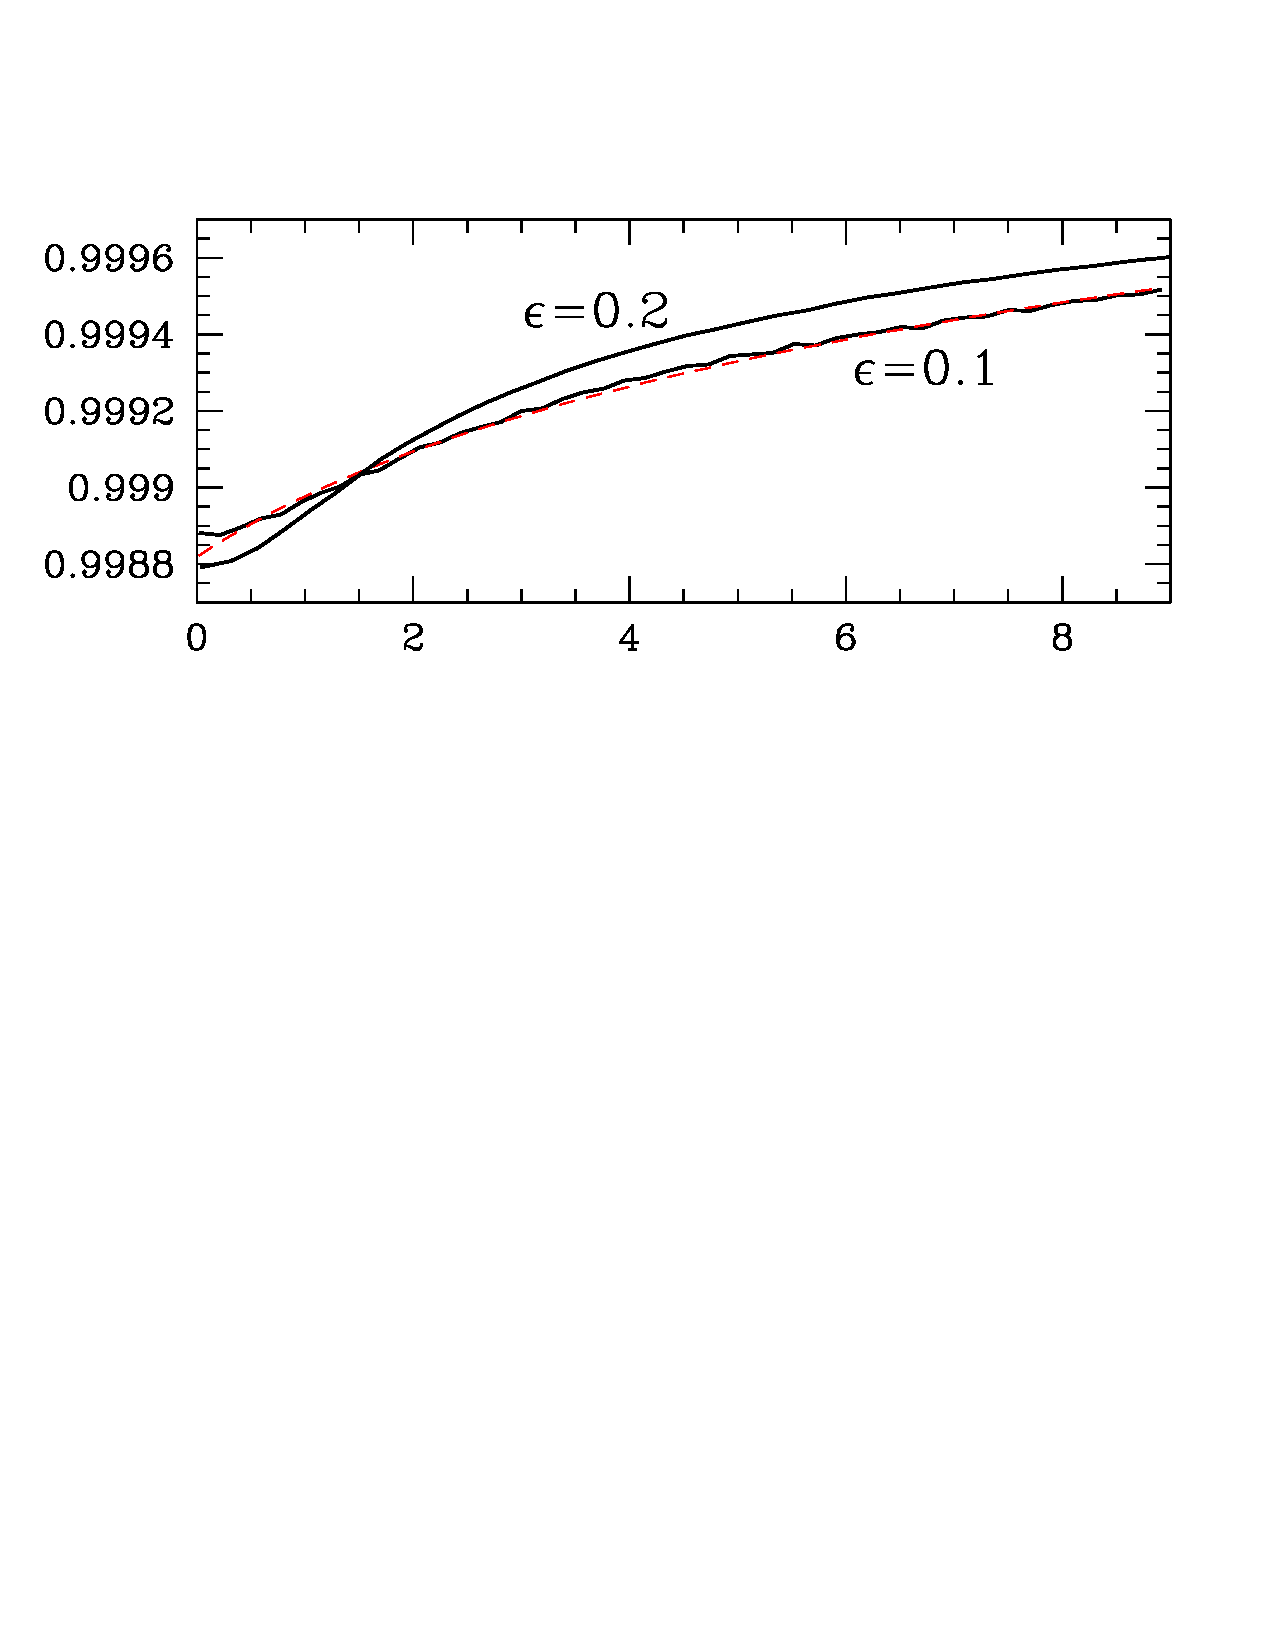
\includegraphics[scale=0.44]{entropymodelnewf1.pdf}
\vskip -3in
\caption{The fractional entropy deficit is plotted against time (in units of the sound-crossing time for the simulation box) for $512^3$ simulations of a perfect radiation fluid with a scale-invariant spectrum of Gaussian perturbations, with {\it rms} fractional density variation $\epsilon=0.1$ and $\epsilon=0.2$ respectively. The dashed curve is a fit to our model in (\ref{eq9}) with $f={1\over 4}$. For $\epsilon=0.2$, the time coordinate is doubled and the entropy deficit rescaled by a quarter. According to the model, to leading order in $\epsilon$, after these scalings the two curves should agree. }
\label{entropyfig}
\end{figure}


 As already mentioned, this entropy deficit is conserved as long as the fluid equations remain valid. Once shocks form, however, they generate entropy at a rate which may be computed as follows~\cite{LL2}. First, the shock strength determines its speed. Local energy-momentum conservation requires that the incoming and outgoing energy and momentum flux balance in the shock's its rest frame. This determines the incoming fluid velocity $v_0$ and the outgoing velocity $v_1$ in terms of the fractional increase $\Delta$ in the density across the shock. One finds  $v_0=\sqrt{(4+3 \Delta)/(4+\Delta)}/\sqrt{3}$ and $v_1=\sqrt{(4+\Delta)/( 4+3 \Delta)}/\sqrt{3}$.  Next, the rest-frame entropy density is directly related to the rest-frame energy density and is therefore enhanced behind the shock front by a factor of $(1+\Delta)^{3\over 4}$. Therefore, the outgoing entropy flux is enhanced relative to the incoming entropy flux by $(1+\Delta)^{3\over 4} (\gamma_1 v_1)/(\gamma_0 v_0) = (1+\Delta)^{1\over 4} \sqrt{(4+\Delta)/(4+3\Delta)}\approx 1 +{1\over 64} \Delta^3$, for small $\Delta$. The entropy density behind the shock is enhanced relative to that in front of the shock by the same factor.  


The entropy production results in the dissipation of shocks. Consider a sinusoidal density perturbation of initial amplitude $\epsilon$ which forms left- and right-moving shocks of strength $\Delta= \epsilon$. Averaging over space, the entropy deficit per unit volume is $-{3\over 64}\Delta^2 s_0$, where $s_0$ is the equilibrium entropy density. The rate of change of this deficit equals the rate at which the shocks generate entropy, which is ${1\over 64}c_s \Delta^3 s_0/\lambda_s$, where $\lambda_s$ is the mean shock separation. Hence, we obtain $\dot{\Delta}=-{1\over 6} (c_s/\lambda_s) \Delta^2$ so that shocks of amplitude $\epsilon$ decay in a time $t_d\sim 6 \lambda_s/(c_s \epsilon)$, larger than the shock formation time by a numerical factor (which, in our simplified model, is $\sqrt{3} \pi\approx 5$ in $d=3$). The shock amplitude decay introduces a short wavelength cutoff in the entropy deficit:
\be
s\approx s_0(1 -{3\over 32} \epsilon^2 \ln\left(\lambda_{2}/(f c_s \epsilon\, t)\right), 
\label{eq9}
\ee
with $f$ a constant ($f={1\over 6}$ in our simplified model). 

We have performed detailed numerical simulations in one, two and three dimensions to check the picture presented above in detail. Fig. \ref{entropyfig} shows a full 3d numerical simulation compared with the prediction in Eq. (\ref{eq9}). The agreement is excellent, providing strong confirmation of the picture we have elaborated, in which the shocks are the dominant mechanism through which the acoustic modes thermalize. 

Not only do shocks generate entropy, shock-shock interactions generate vorticity. As we have already explained, since the usually assumed initial conditions are irrotational, as long as the fluid equations hold vorticity can never be generated. Shocks provide a way out, generating vorticity in a precisely calculable amount. For example, one can find a stationary solution representing two shocks intersecting on a line, leaving a ``slip sheet'' behind it across which the tangential component of the velocity is discontinuous. The strength of the tangential discontinuity (and hence the vorticity) may be shown to be proportional to $\Delta^3$, where $\Delta$ is the shock amplitude. More generally, non-stationary configurations can generate parametrically larger vorticity and indeed, it is conceivable that in rare localized regions fully developed turbulence may occur. Note that for a perfect conformal fluid, the dispersion relation is linear in $k$. Unfortunately, in this case, standard methods for studying the onset of wave turbulence do not apply (see, {\it e.g.} Ref. \cite{ZLF}) . 
 
There are a number of possible observational consequences of shock formation in the early universe: (i) the formation of primordial vorticity, and consequent magnetic fields, (ii) local departures from thermal equilibrium, of potential relevance to baryogenesis, (iii) the seeding of small-scale isocurvature perturbations and inhomogeneities relevant to primordial nucleosynthesis and (iv) the emission by shock-shock collisions of short wavelength gravitational waves which may be detectable today. In principle, each of these may produce an observable signal: all are currently under investigation. 
         
\vskip .2in        
\noindent
{\it Acknowledgments:} We thank Dick Bond, Job Feldbrugge, Luis Lehner, Dam Son and Ellen Zweibel for valuable discussions and encouragement. Research at Perimeter Institute is supported by the Government of Canada through Industry Canada and by the Province of Ontario through the Ministry of Research and Innovation. 

\begin{thebibliography}{99}

\bibitem{Gielen} Steffen Gielen and Neil Turok, preprint arXiv:XXX (2015). 

\bibitem{weblink} https://github.com/PerimeterInstitute/shocks-in-the-early-universe/wiki



\bibitem{penturoklong} J. Feldbrugge, Ue-Li Pen and Neil Turok, in preparation (2015). 

\bibitem{ZLF} V.E.~Zakharov, V.S.~L'vov, G.~Falkovich, {\em Kolmogorov Spectra of Turbulence I: Wave Turbulence}, Springer-Verlag, 1992. See discussion on p. 66.



\bibitem{moore} 
  P.~B.~Arnold, G.~D.~Moore and L.~G.~Yaffe,
  %``Transport coefficients in high temperature gauge theories. 1. Leading log results,''
  JHEP {\bf 0011}, 001 (2000)
  [hep-ph/0010177].

\bibitem{foot1} We use units in which the speed of light is unity. 

\bibitem{foottilt} We ignore the modest effect of scalar tilt on the power spectrum. For example, extrapolating the observed $CMB$ spectral tilt $n_s-1\approx .033$ reduces the scalar amplitude on the Hubble radius at the electroweak temperature by less than a factor two. 


\bibitem{LL} L.~D.~Landau and E.~M.~Lifshitz, {\it Fluid Mechanics}, Pergamon 1987, Sec. 103. 
\bibitem{LL2} {\it Ibid}, Sec. 135. 


\bibitem[Trac 
\& Pen(2003)]{trac} Trac, H., \& Pen, U.-L.\ 2003, \pasp, 115, 303 




\end{thebibliography}

\end{document}
